%************************************************
\chapter{Experimental Setup}
\label{ch:detector}
%************************************************

\section{Introduction}
\label{sec:detector_introduction}

Our experimental data was collected from the ATLAS particle detector in the Large Hadron Collider (LHC).
The following section will introduce LHC and the ATLAS particle detector.

\section{The Large Hadron Collider}
\label{sec:detector_LHC}

The Large Hadron Collider (LHC) was built in the border between France and Switzerland by the European Organization for Nuclear Research (CERN).
It is a circular particle collider under the ground with circumference 27 km.
Two beams of protons will be accelerated in opposite directions, to almost the speed of light, and then these two beams will collide with each other at the collision point.
The energy of each beam is 6.5 TeV, and hence the center-of-mass energy of the two beams $\sqrt{s}$ is 13 TeV, which is the energy used in this experiment.
This energy is equivalent to the speed that the beam will circulate the ring 11,245 times per second.
Under this high energy, new physics phenomena will happen, including SUSY.
Figure \ref{fig:detector_LHC_accelerator_complex} shows the schematic diagram of the CERN accelerator complex, which contains a series of accelerators, from low energy to high energy.
The dark blue big circle in figure \ref{fig:detector_LHC_accelerator_complex} represents the LHC, on which there are 4 particle detectors at 4 different interaction points (yellow points): ATLAS, CMS, LHCb and ALICE.
By analyzing these collisions, we can have a deeper understanding of the laws of nature.

\begin{figure}
\centering
\includegraphics[width=\textwidth]{data/photo/detector/accelerator_complex.png}
\caption{The schematic diagram of the CERN accelerator complex, which shows a series of accelerators and facilities. \cite{complex}}
\label{fig:detector_LHC_accelerator_complex}
\end{figure}

Before the beam is injected into LHC, the protons need to be accelerated by a series of accelerators.
The journey of the protons starts from a tank of hydrogen gas.
The proton and the electron are separated by a electric field.
The protons are then accelerated to 50 MeV by Linac2, which is a linear accelerator.
The beam is then injected to the second accelerator called the Proton Synchrotron Booster (PSB), which accelerates the beam to 1.4 GeV.
The beam is then injected to the third accelerator called the Proton Synchrotron (PS), which pushes the beam to 25 GeV.
The beam is then injected to the fourth accelerator called the Super Proton Synchrotron (SPS), which further pushes the beam to 450 GeV.
Finally, the beam is injected to the two beam pipes of the LHC.
One of the beam moves in clockwise direction, while another beam moves in anti-clockwise direction.
Two beams will be collided at the collision point inside the ATLAS detector.
\cite{accelerator}

The circular path of the proton beam is maintained by many superconducting electromagnets along the LHC tunnel.
There are 1232 main magnetic dipoles, and each of them generates a large magnetic field of 8.3 T.
In order to generate such a high magnetic field, the coils need to have very high currect of 11,080 A, and hence supercoducting coil need to be used, to reduce the heat loss due to the electrical resistance.
The material of supercoducting coil is niobium-titanium (NbTi).
To reach the condition for supercoductivity, the electromagnets operate at a very low temperature of 1.9 K.
There are also 392 magnetic quadrupole to squeeze the proton beam, so that the chance of proton-proton collision will be higher.
\cite{supermagnet,cryogenics}

The protons in the beam are grouped into different bunches, and there are about $10^{11}$ protons in each bunch.
The time-spacing between two adjacent bunches is 25ns (or 50 ns in the old configuration).
This means that in each 25 ns, two bunches are collided at the collision point.
For each bunch collision, there are about 10 to 50 proton-proton interaction.
Hence, about $10^9$ proton-proton collisions are produced in one second.

The interacting rate for a physics proccess $\frac{dN}{dt}$ is the product of the cross section of that physics proccess $\sigma$ and the instantaneous luminosity $\mathcal{L}$.
\begin{equation}
\frac{dN}{dt} = \sigma \mathcal{L}
\end{equation}
The instantaneous luminosity $\mathcal{L}$ is a measure of the interacting rate of two protons at the collision point, which is related to the density of the protons and the speed of the protons.
The instantaneous luminosity in this experiment is about $10^{34}$ cm$^{-2}$ s$^{-1}$ (or 10 nb$^{-1}$ s$^{-1}$).

\section{ATLAS detector}
\label{sec:detector_ATLAS}

A Toroidal LHC ApparatuS (ATLAS) is the particle detector used in this experiment \cite{ATLAS_doc}.
Figure \ref{fig:detector_ATLAS} shows the main components of the ATLAS detector.
\begin{figure}
\centering
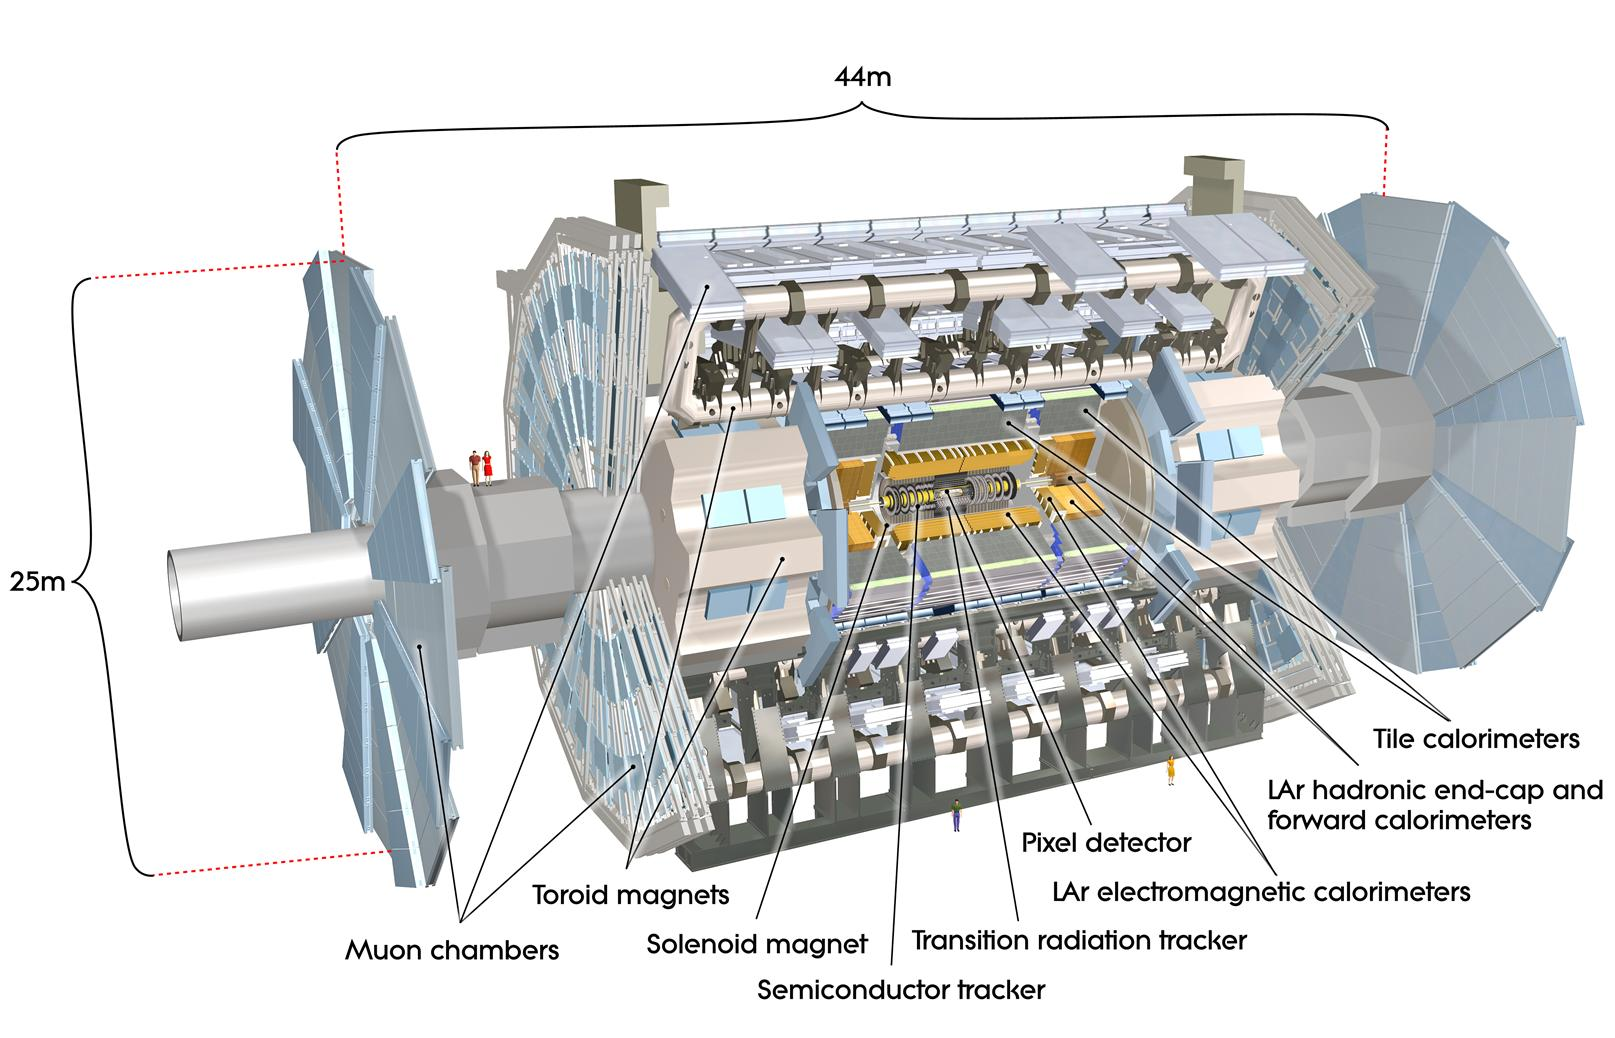
\includegraphics[width=\textwidth]{data/photo/detector/ATLAS.jpg}
\caption{The cut-away view of the ATLAS detector. It is 25m high and 44m long. \cite{ATLAS_photo}}
\label{fig:detector_ATLAS}
\end{figure}
The ATLAS detector is a general purpose particle detector, which is consisted of 3 main components: the inner detector, the calorimeter and the muon spectrometer.
Figure \ref{fig:ATLAS_particles} shows how the ATLAS distinguishes different types of particle. The inner detector can detect the paths of the charged particles.
Photons and electrons will deposit most of their energy in the electromagnetic calorimeter, and finally stop by it.
Hadrons(including protons and neutrons) and mesons will similarly stop by the hadronic calorimeter.
Only muons and the neutrinos can reach the outermost muon spectrometer, but only muons can be detected by the muon spectrometer.
Nearly all neutrinos will escape the whole ATLAS detector, which leads to some missing energy.
In this design, different particles can be identified due to their signature in different parts of ATLAS.
\begin{figure}
\centering
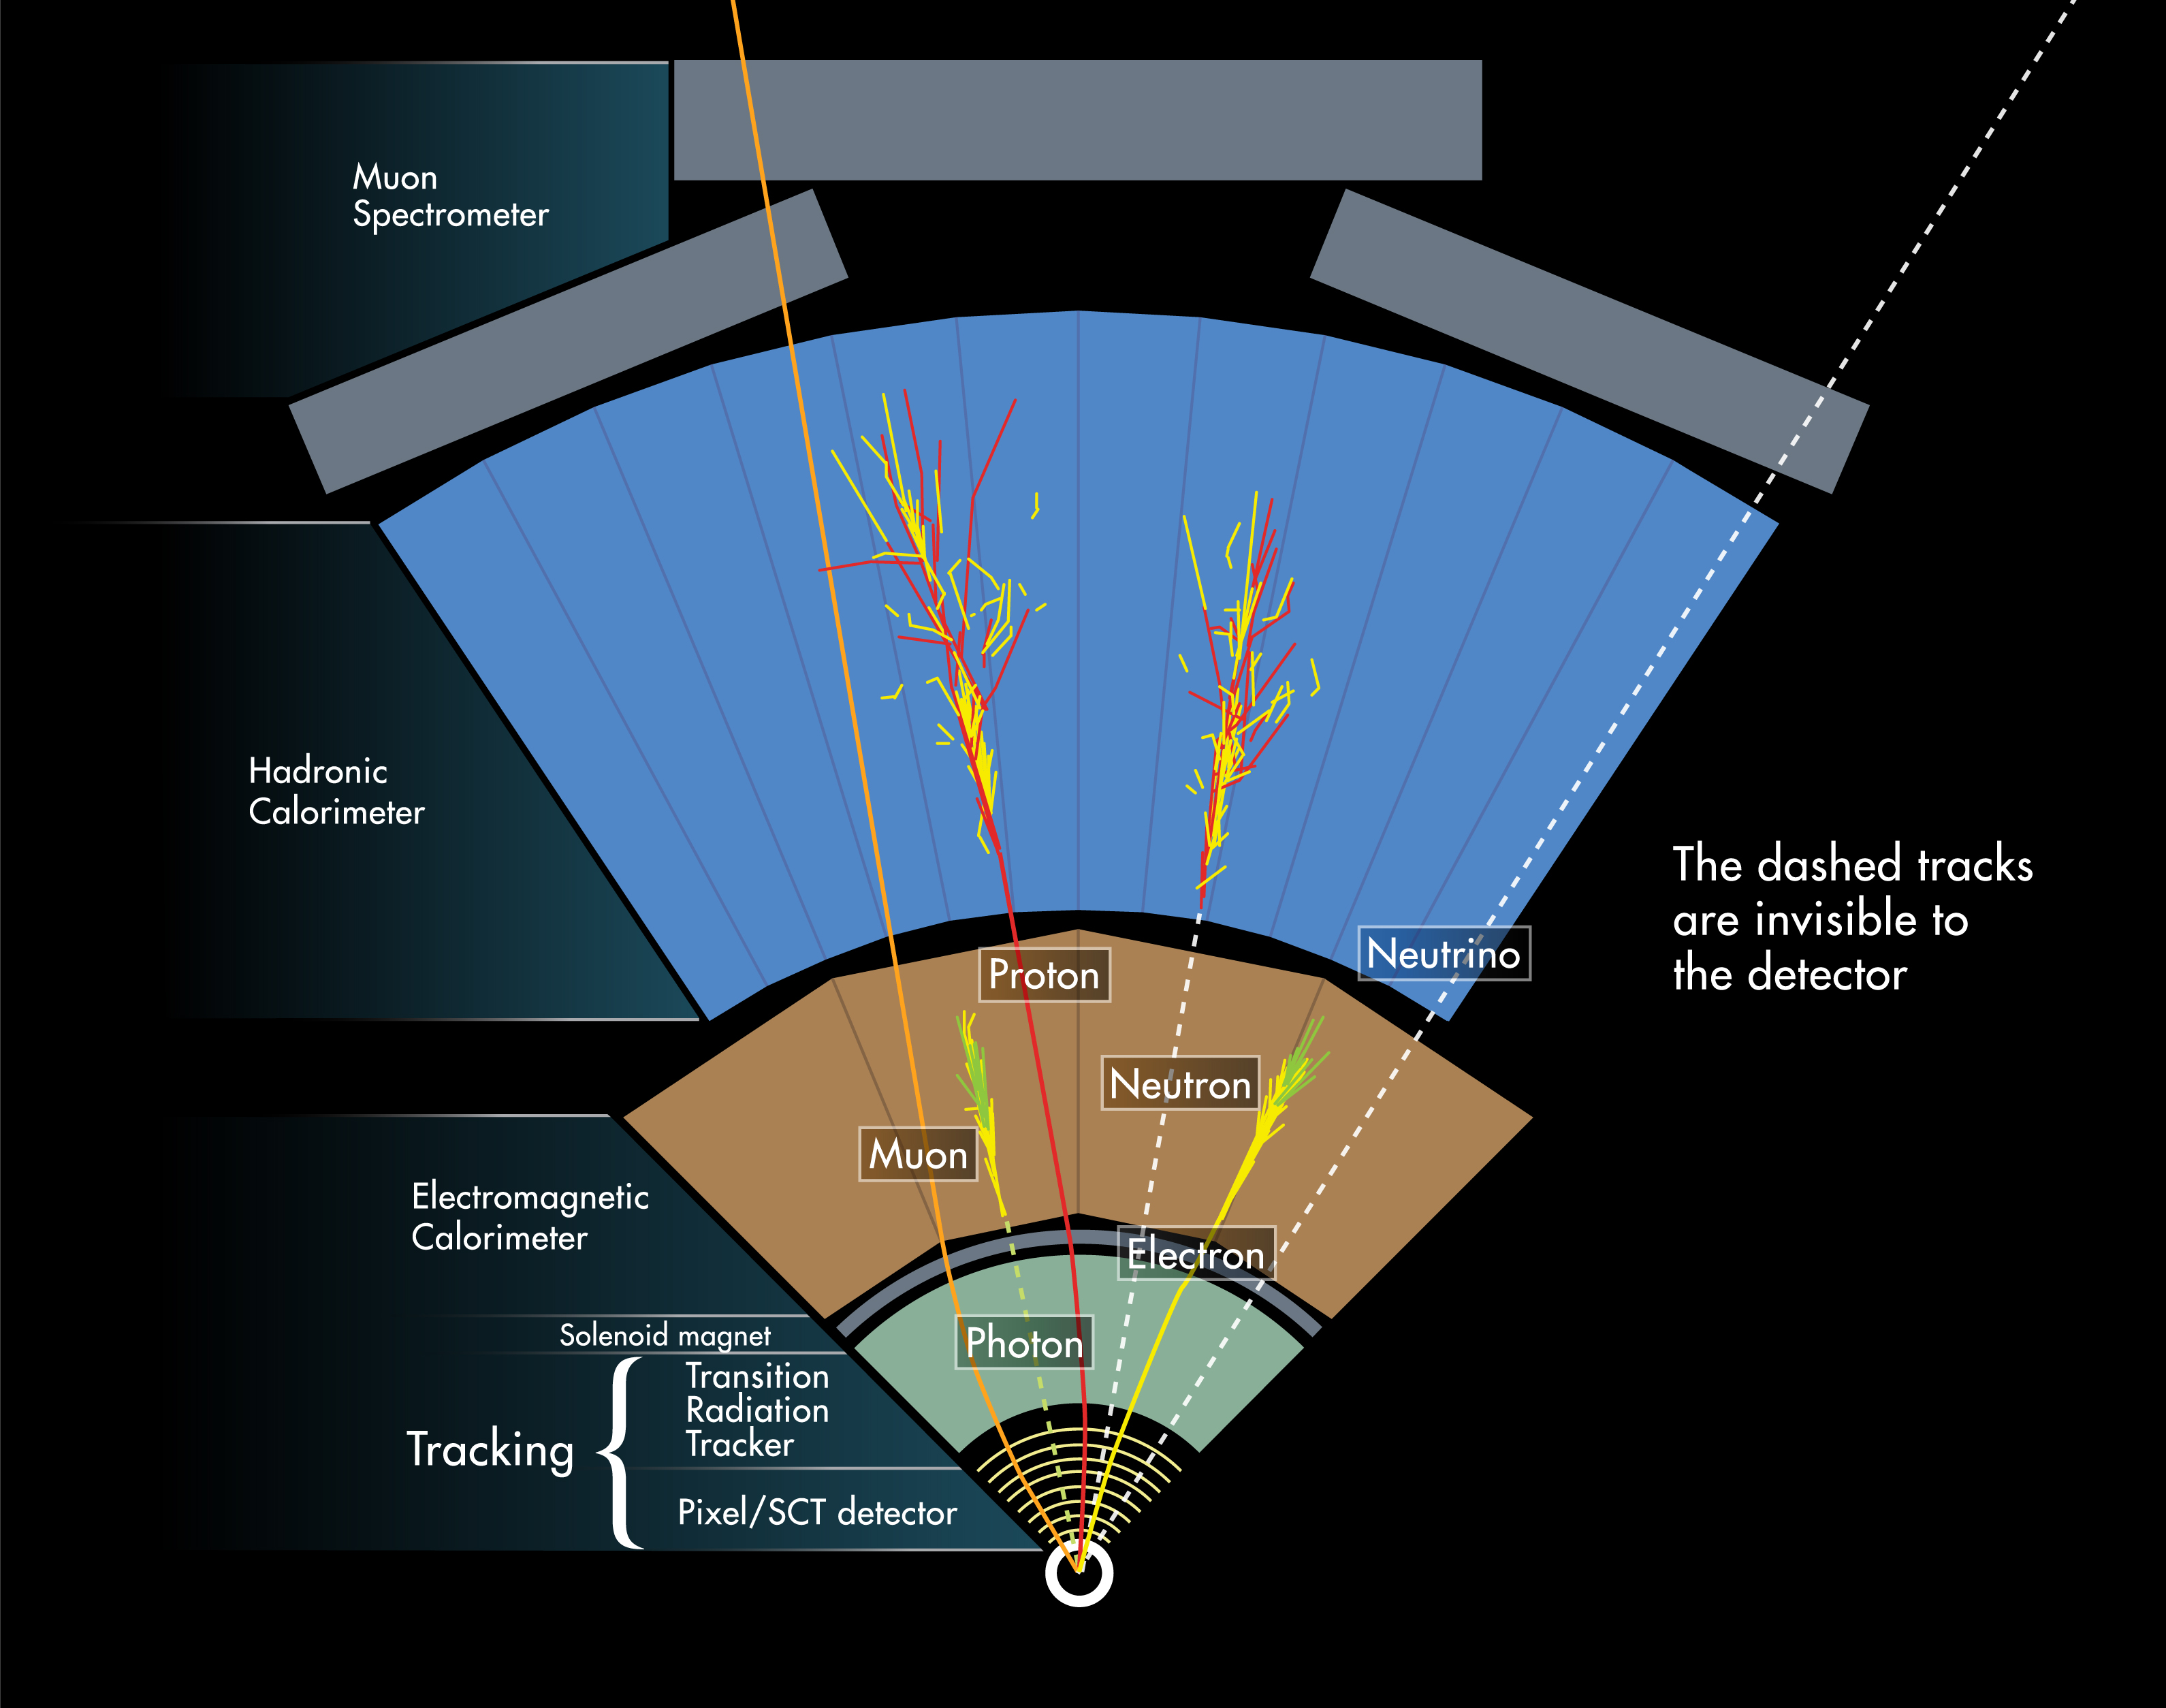
\includegraphics[width=\textwidth]{data/photo/detector/ATLAS_particles.jpg}
\caption{The cross section of the ATLAS detector. This shows different components of the ALTAS and how ATLAS detect different types of particles \cite{ATLAS_particles}}
\label{fig:ATLAS_particles}
\end{figure}

\subsection{coordinate system}
The nominal collision point is defined as the origin of the coordinate system.
The z-axis is along the beam dirention.
The positive x-asix is pointing to the centre of the LHC ring.
The positive y-asix is in the upward direction.
The azimuthal angle $\phi$ and the polar angle $\theta$ are defined as usual in the spherical coordinate system.
The pseudorapidity $\eta$ is defined as:
\begin{equation}
\eta = - \ln \Big( \tan \frac{\theta}{2} \Big)
\end{equation}
The distance $\Delta R$ in the pseudorapidity-azimuthal angle space is defined as:
\begin{equation}
\Delta R = \sqrt{(\Delta \phi) ^2 + (\Delta \eta) ^2}
\end{equation}
The ATLAS detector has a reflection symmetry about the x-y plane.

\subsection{magnetic system}
There is a thin superconducting solenoid magnet around the inner detector, which generates a 2 T magnetic field inside the inner detector.
There are also 3 large superconducting toroids around the calorimeter: one for barrel and two for end-caps.
All these magnets are shown in figure \ref{fig:detector_ATLAS}.

\subsection{The inner detector}
The inner detector is a particle tracker.
It mainly detects the tracks of charged particles and has good performance for measuring the momentum of the charged particles and locating the position of the vertices.
Figure \ref{fig:detector_inner_whole} shows the whole structure of the inner detector.
The inner detector consists of 3 sub-detectors from inner to outer: the pixel detector, the silicon microstrip tracker (SCT) and the transition radiation tracker (TRT).
Each part further divides into two parts: the barrel region with smaller $|\eta|$ and the end-cap region with larger $|\eta|$.
Figure \ref{fig:detector_inner_detail} shows the distances R from the beam for the 3 sub-detectors, and figure \ref{fig:detector_inner_size} shows the shapes and the orientations of each sensor and the $\eta$ coverage, in both the barrel and the end-cap regions.
The $\eta$ coverage for the inner detector is $|\eta| < 2.5$.
The shapes and the orientations of the sensors are different in the barrel and the end-cap regions.
In the barrel region, the shape and the orientation of the sensors is concentric cylinder shells around the beam axis, while in the end-cap region, they are disks perpendicular to the beam axis.
\begin{figure}
\centering
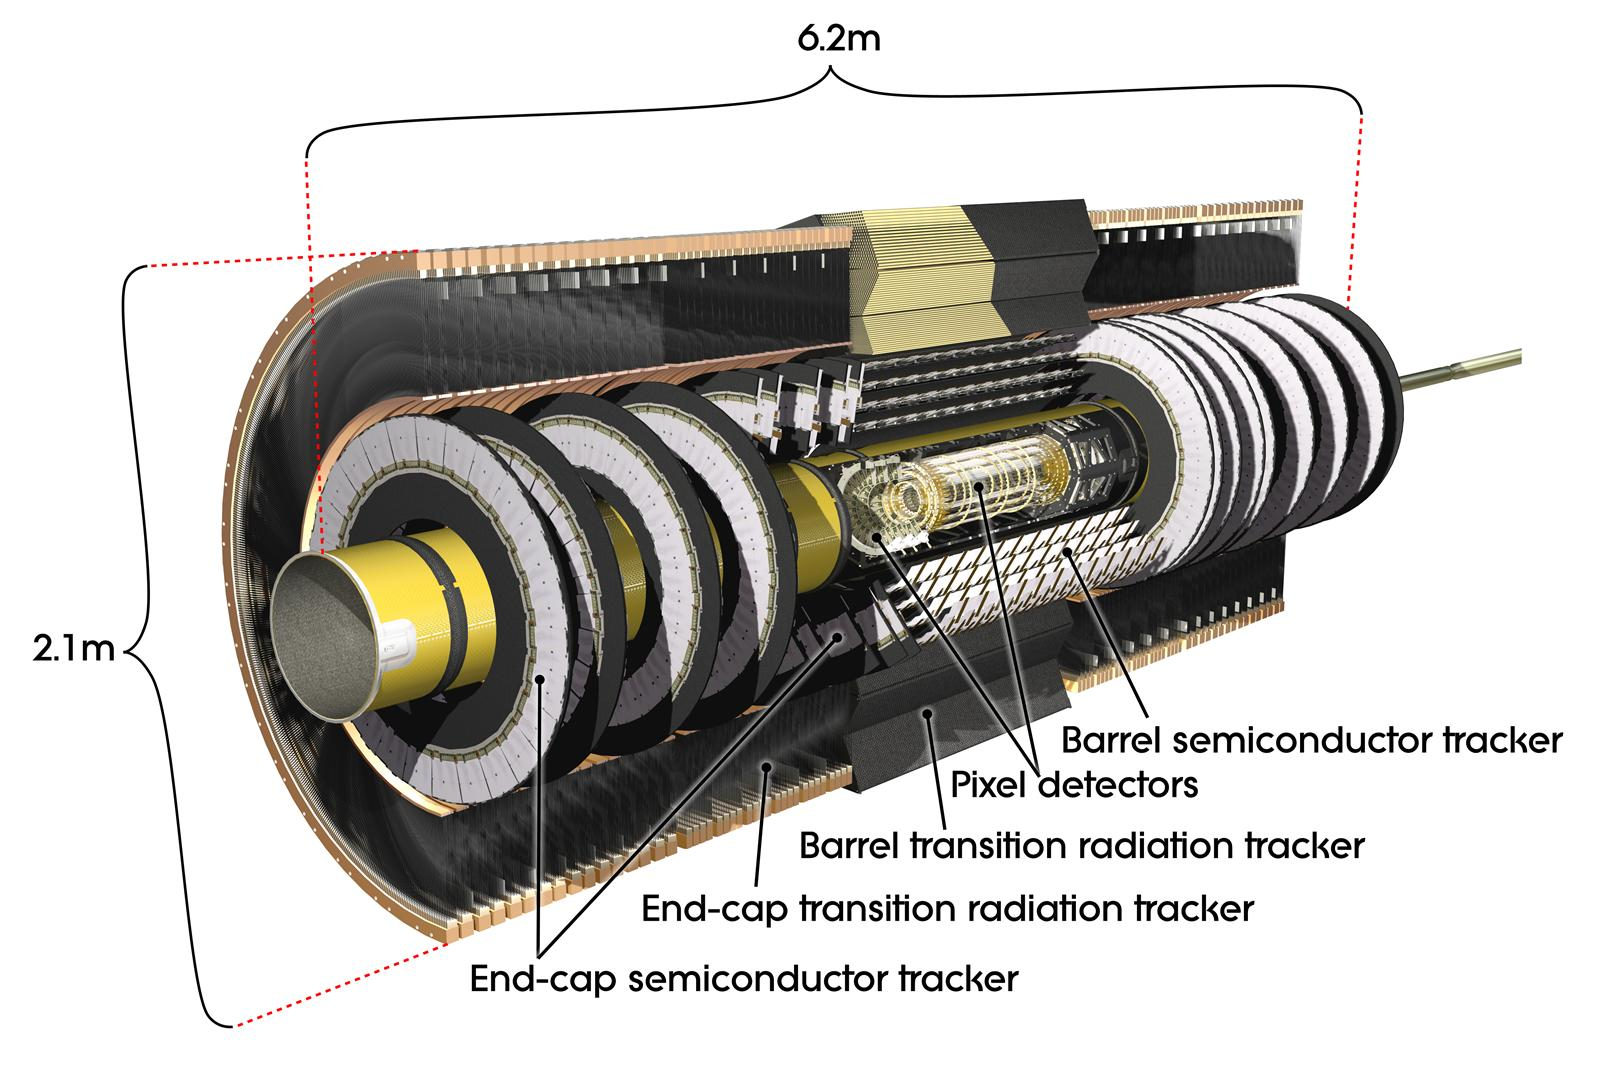
\includegraphics[width=\textwidth]{data/photo/detector/inner_whole.jpg}
\caption{The whole structure of the ATLAS inner detector. \cite{inner_photo}}
\label{fig:detector_inner_whole}
\end{figure}
\begin{figure}
\centering
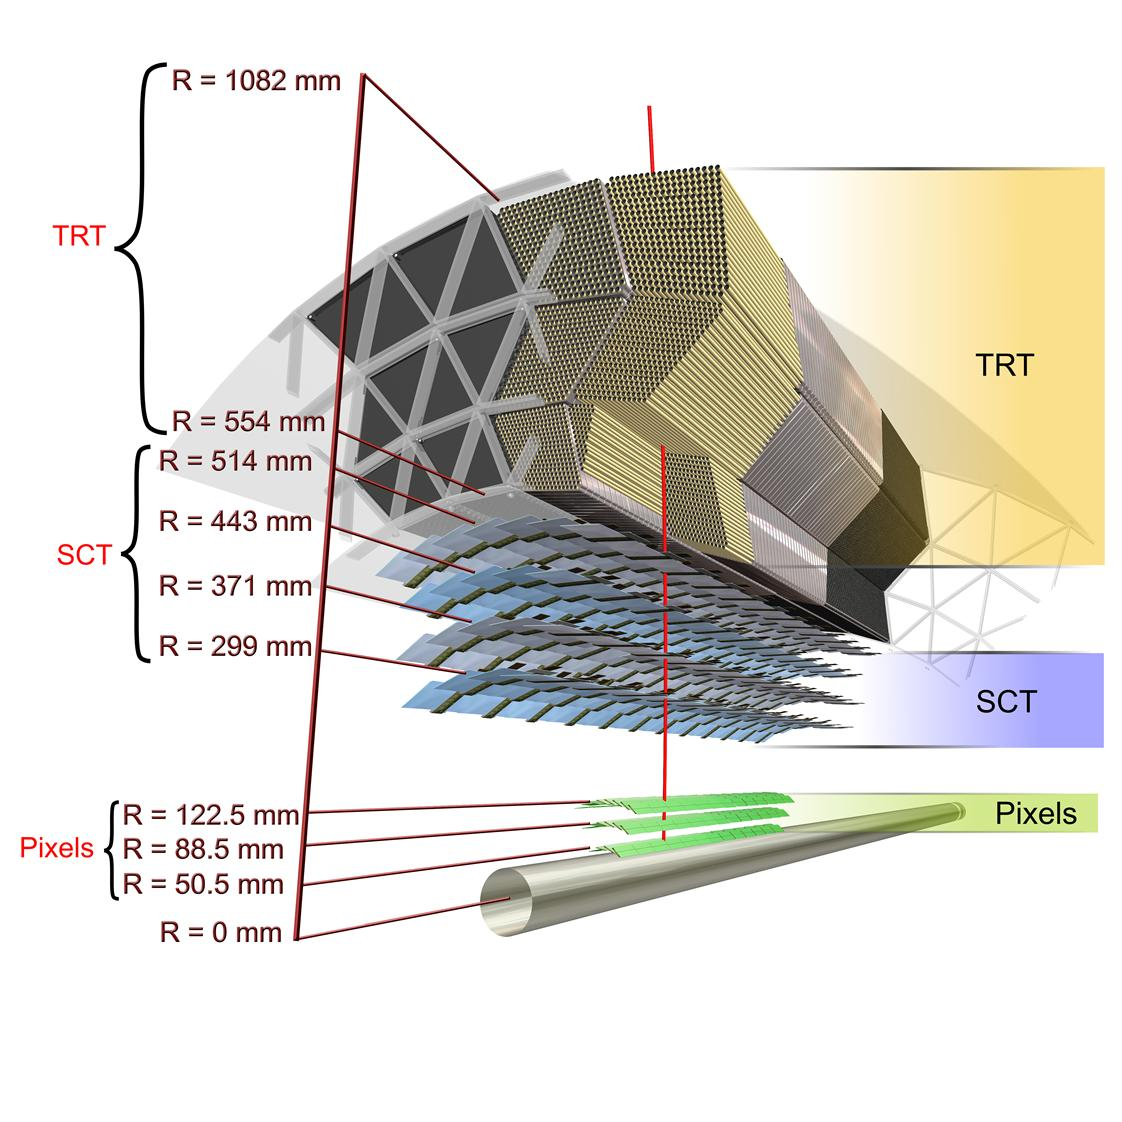
\includegraphics[width=\textwidth]{data/photo/detector/inner_detail.jpg}
\caption{The distances R from the beam for the 3 components: pixel, SCT and TRT. \cite{inner_photo}}
\label{fig:detector_inner_detail}
\end{figure}
\begin{figure}
\centering
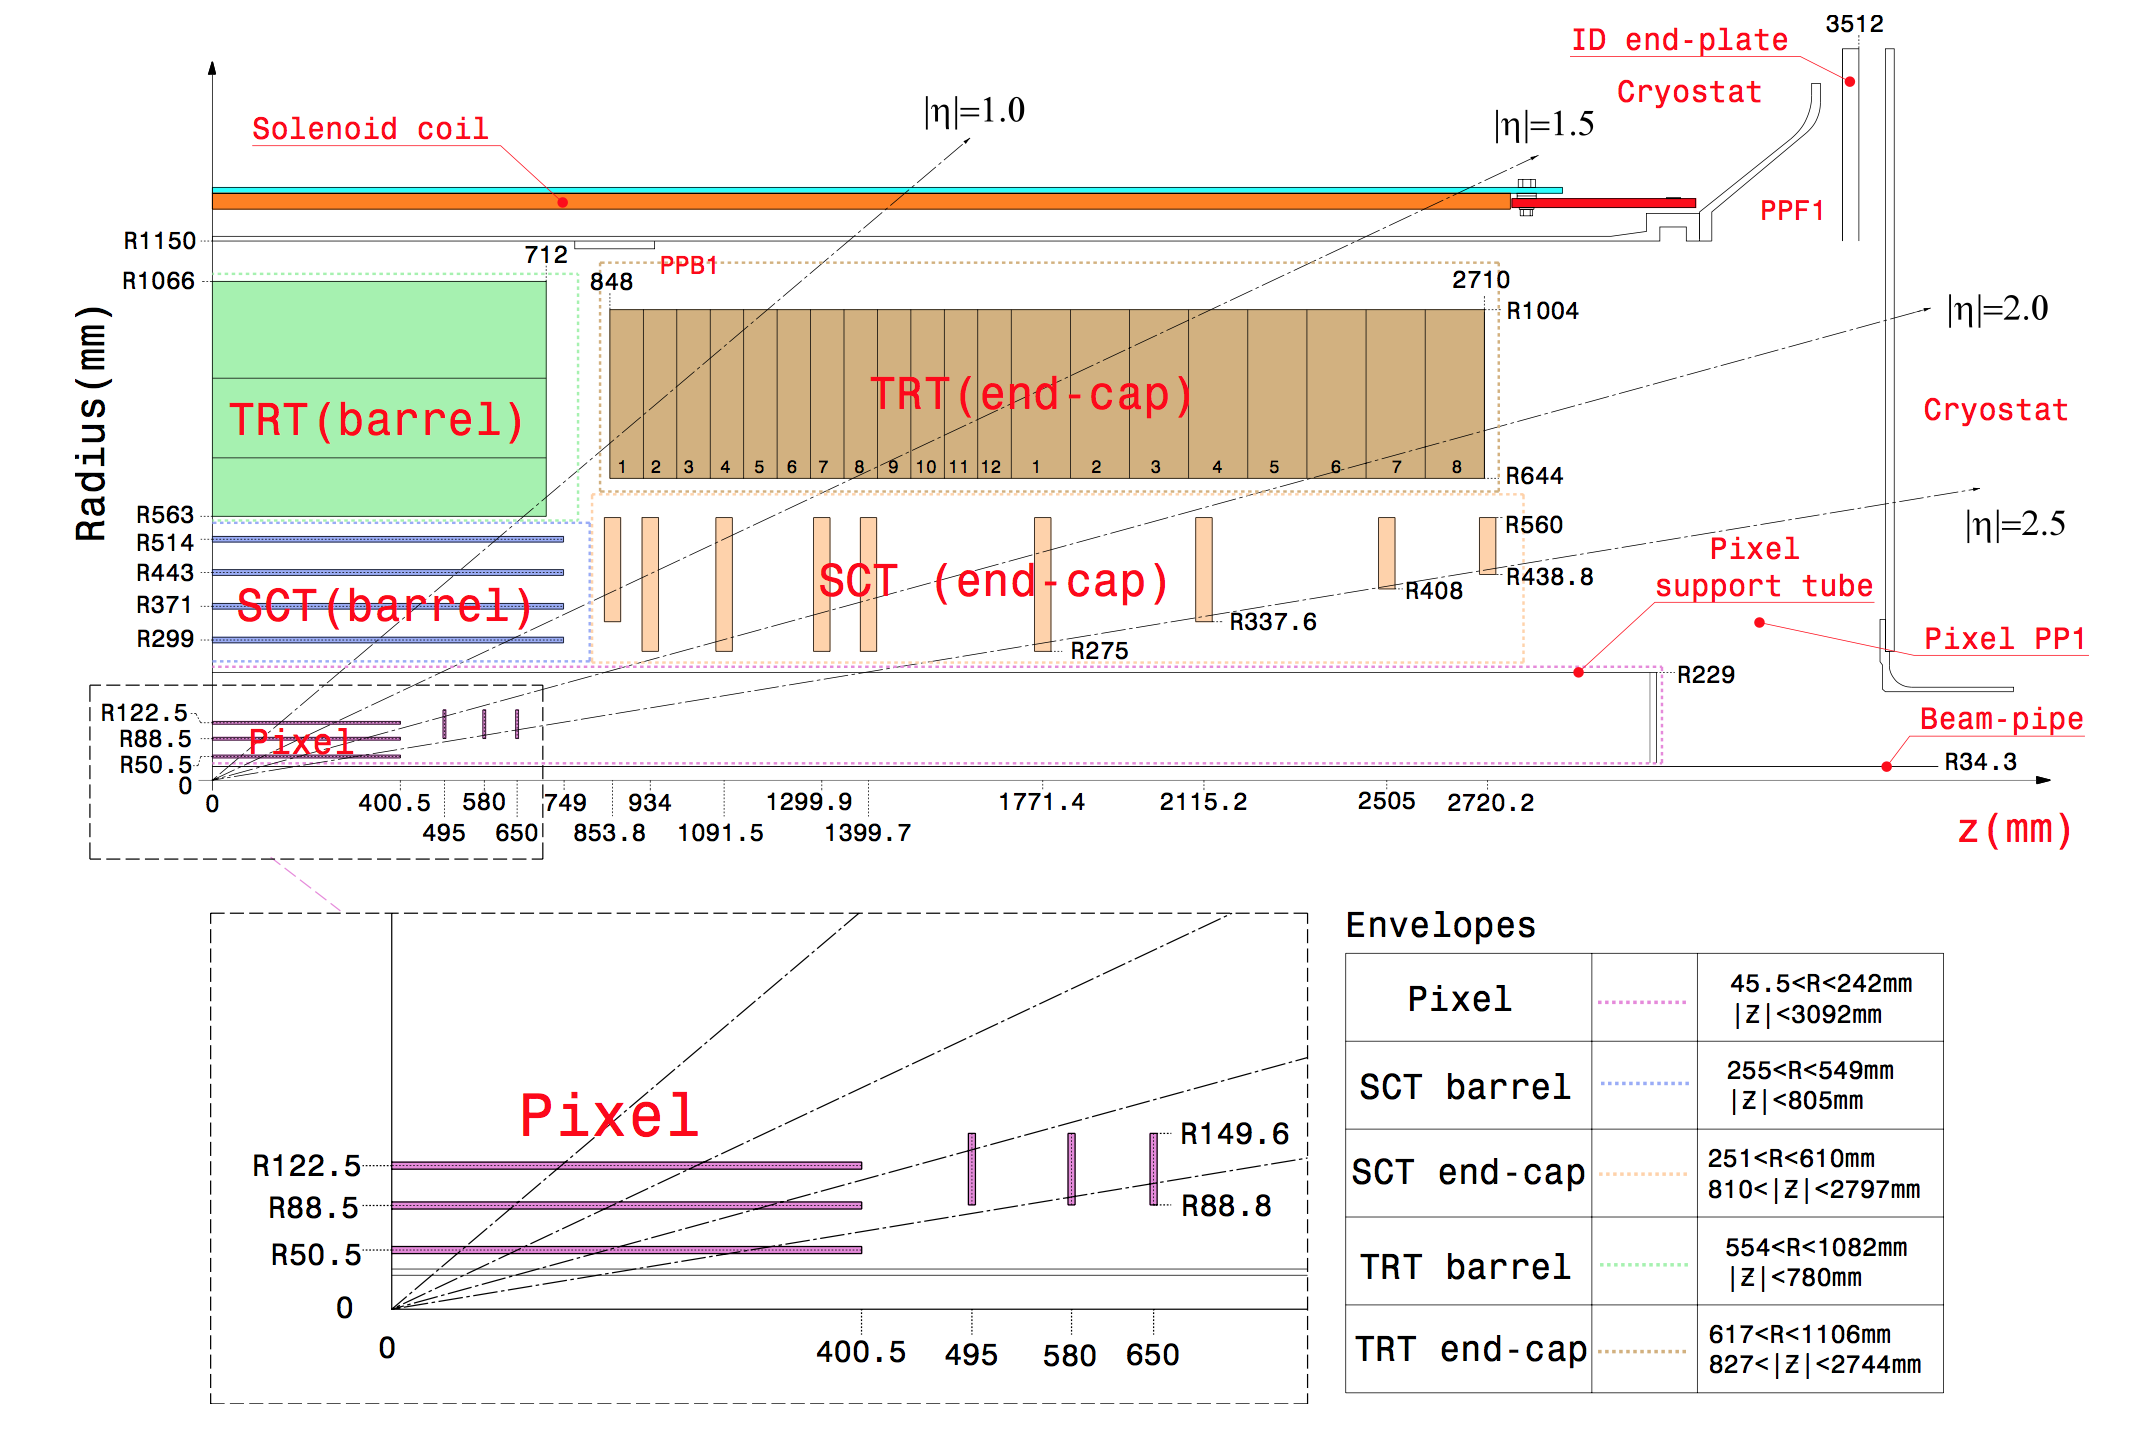
\includegraphics[width=\textwidth]{data/photo/detector/inner_size.png}
\caption{The shapes, the orientations and the $\eta$ coverage for each sensor. \cite{ATLAS_doc}}
\label{fig:detector_inner_size}
\end{figure}

The precision tracking detectors (pixels and SCT) has high resolution in space by using discrete space-points to detect the track of a charged particle, with the cutting-edge technology, in order to achieve the good performance of the inner detector.
When the particle moves inside the inner detector, there are, in average, 36 hits per one track.
By recording the positions of these hits, the path of the particle can be reconstructed.
The whole inner detector is immersed in a 2 T magnetic field generated by the solenoid magnet, and hence the path of any charged particles will be bent.
By measuring the curvature of the path, the charge and momentum of the particle can be measured.
The equation for the circular path is
\begin{equation}
\frac{d\mathbf{p}}{dt} = q(\mathbf{v} \times \mathbf{B})
\end{equation}
where the relativistic momentum $\mathbf{p} = \gamma m \mathbf{v}$.
\begin{align}
\frac{d\mathbf{p}}{dt} &= q( \frac{\mathbf{p}}{\gamma m} \times \mathbf{B}) \\
&= \frac{q}{\gamma m} (\mathbf{p} \times \mathbf{B})
\end{align}
From this equation, we can get the angular frequence $\omega$,
\begin{align}
\omega &= \frac{qB}{\gamma m} \\
\frac{v}{r} &= \frac{qB}{\gamma m} \\
\frac{1}{r} &= \frac{qB}{\gamma m v} \\
\frac{1}{r} &= \frac{qB}{p} \\
p &= rqB
\end{align}
By this equation, we can calculate the momentum of the particle, from the curvature of track $1/r$, the charge and the magnetic field strength.

\subsubsection{Pixel detector}
As shown in figure \ref{fig:detector_inner_size}, there are 3 layers of cylinder in the barrel region, and 3 layers of disk for each end-cap region.
There are in total 1744 modules in the pixel detectors.
Each module is identical, and has the size of 19mm$\times$63mm, and 250 $\mu$m thick.
The module has 47232 pixels, which has size of 50$\mu$m$\times$400$\mu$m, and hence there are in total 80 million pixels for the whole pixel detector.
Each pixel has the accuracy of 10$\mu$m$\times$115$\mu$m.
The sensor is using planar n$^{+}$-in-n type of silicon, with n$^{+}$-type at the readout side and n-type at another side.

\subsubsection{SCT}
As shown in figure \ref{fig:detector_inner_size}, there are 4 layers of cylinder in the barrel region, and 9 layers of disk for each end-cap region.
There are in total 4088 modules in the SCT, with the thickness of 285 $\mu$m.
There are in total 6.3 million pixels for the SCT.
Each pixel has the accuracy of 17$\mu$m$\times$580$\mu$m.
The sensor is using planar p-in-n type of silicon.

\subsubsection{TRT}
136 TRT modules.
TRT in the outer part is to produce and detect the transition radiation from the particle. TRT comprises many layers of gaseous straw tube elements interleaved with transition radiation material.
Each pixel has the accuracy of 130$\mu$m.

\subsection{Calorimeter}
\begin{figure}
\centering
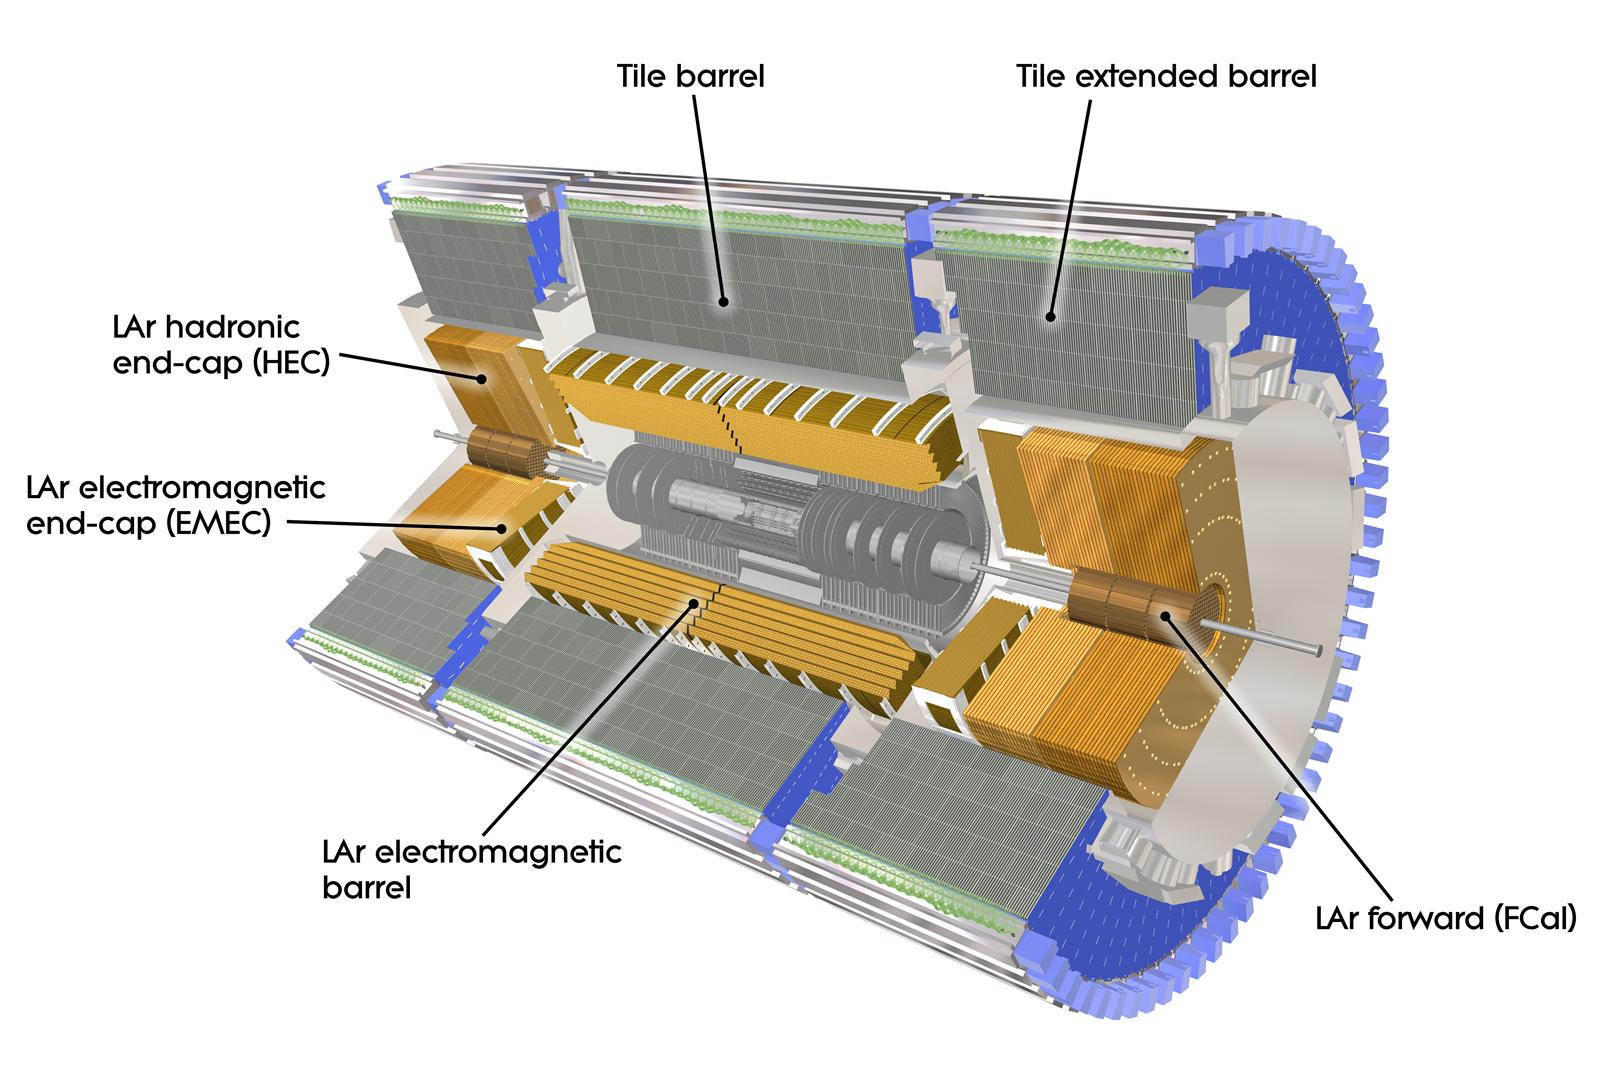
\includegraphics[width=\textwidth]{data/photo/detector/calorimeter_whole.jpg}
\caption{whole calorimeter \cite{calorimeter_whole}}
\label{fig:calorimeter_whole}
\end{figure}

\subsubsection{Electromagnetic calorimeter}

\subsubsection{Hardronic calorimeter}

\subsection{Muon Spectrometer}
\begin{figure}
\centering
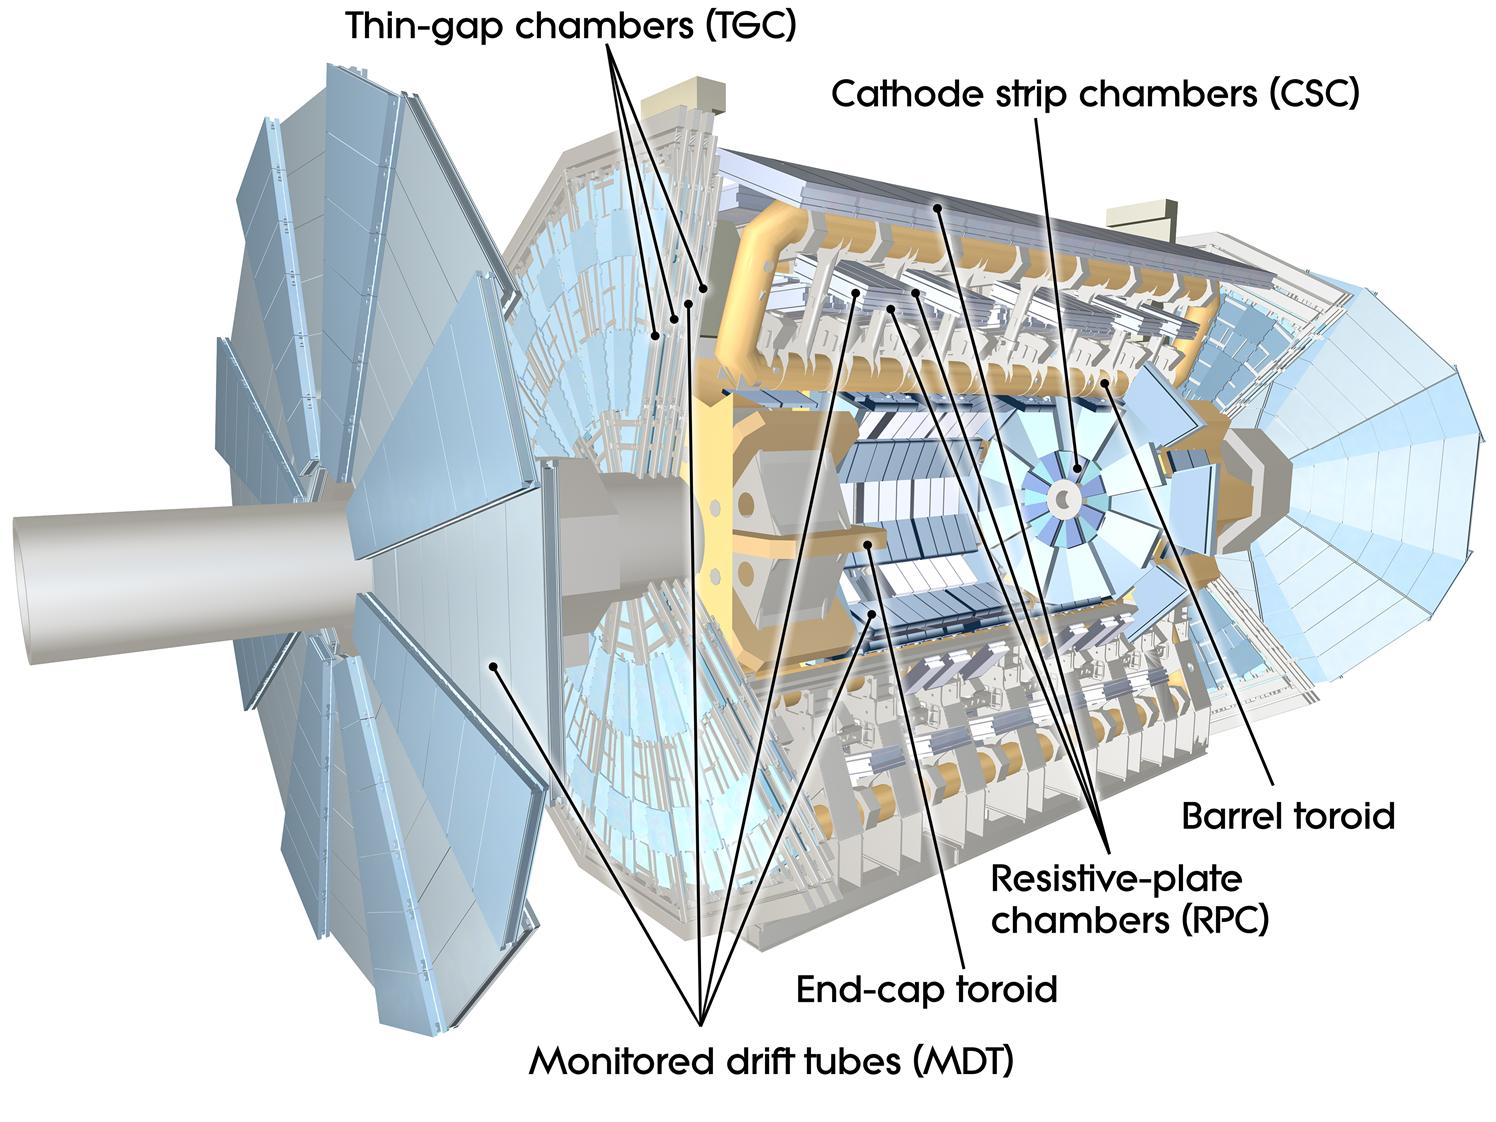
\includegraphics[width=\textwidth]{data/photo/detector/muon_spectrometer.jpg}
\caption{muon spectrometer \cite{muon_spectrometer}}
\label{fig:muon_spectrometer}
\end{figure}
